\documentclass[aspectratio=169]{beamer}

% Options Beamer.
\usetheme{Madrid}
\usecolortheme{whale}
\usefonttheme[onlymath]{serif}
\setbeamertemplate{section in toc}{\inserttocsectionnumber.~\inserttocsection}
\setbeamertemplate{subsection in toc}{%
  \hspace{1.2em}{\color{black}\rule[0.3ex]{3pt}{3pt}}~\inserttocsubsection\par}
\usepackage{caption}
\usepackage{pgfplots}
\usepackage{listings}
\usepackage{lstautogobble} % Provides autogobble, which is useful to remove indentation based on first line

\lstset{ %
  language=C,
  numbers=left,
  numberstyle=\tiny,
  stepnumber=1,
  numbersep=5pt,
  breaklines=true,
  autogobble=true, % Removes indentation based on first line
}
\pgfplotsset{compat=1.17}

% Personnalisation de la première page.
\title{\LARGE Apprentissage non-supervisé pour l'estimation de champs de
déformation à la surface de matériaux soumis à des
contraintes mécaniques}
\author{Projet Recherche - Oscar Egreteau\\[1em] Sous la supervision de F.Sur, LORIA}

% \titlegraphic{
%     \centering
%     \includegraphics[height=2.3cm]{logo.png}
%     \hspace{2.5cm}
%     \includegraphics[height=2.3cm]{logobis.jpeg}
% }
\date{9 janvier 2026}


\setbeamertemplate{footline}{
  \leavevmode%
  \hbox{%
  \begin{beamercolorbox}[wd=.33333\paperwidth,ht=2.5ex,dp=1ex,left]{author in head/foot}%
    \centering Oscar Egreteau
  \end{beamercolorbox}%
  \begin{beamercolorbox}[wd=.33333\paperwidth,ht=2.5ex,dp=1ex,center]{title in head/foot}%
    Projet Recherche
  \end{beamercolorbox}%
  \begin{beamercolorbox}[wd=.33333\paperwidth,ht=2.5ex,dp=1ex,right]{date in head/foot}%
    \centering\insertframenumber{} / \inserttotalframenumber
  \end{beamercolorbox}}%
  \vskip0pt%
}

\begin{document}

\begin{frame}
    \titlepage
\end{frame}

\begin{frame}
    \frametitle{Sommaire}
    \tableofcontents
\end{frame}

\section{Introduction}
\begin{frame}
    \frametitle{Introduction}
    \begin{itemize}
    \item Analyse du flot optique pour estimer le champ de déformation de matériaux
    \item Apprentissage non supervisé car difficulté d'avoir une réalité terrain : pas possible de connaître le champ de déformation sur un matériau sans l'utilisation d'une méthode d'estimation numérique.
\end{itemize}
\begin{figure}
        \centering 
        \includegraphics[height=4cm]{Images/intro.png}
        \caption*{Un exemple de champ de déformation}
    \end{figure}
\end{frame}


\section{Flot Optique}
\subsection{Définition}

\begin{frame}
    \frametitle{Flot Optique}
    \framesubtitle{Définition}
    Le flot optique est un champ de vecteurs qui représente le déplacement des pixels entre deux images consécutives. Son calcul repose sur une hypothèse fondamentale, celle de la luminosité constante.\\
    \begin{figure}
        \centering
        \includegraphics[scale=0.22]{Images/vag.png}
        \caption*{Un exemple de flot optique}
    \end{figure}
\end{frame}

\begin{frame}
    \frametitle{Flot Optique}
    \framesubtitle{Définition}
    Le flot optique $\bold{u}=(u_1,u_2)$ est régi par l'équation suivante, obtenue en en dérivant l'hypothèse de la luminosité constante ($\forall t\geq 0, \ I(t,x_1(t),x_2(t))=I_0$) :
    \begin{align*}
        \dfrac{\partial I}{\partial t}+\nabla I\cdot \bold{u} &= \dfrac{\partial I}{\partial t}+\dfrac{\partial I}{\partial x}u_1+\dfrac{\partial I}{\partial t}u_2\\
        &=0
    \end{align*}
    Qui est un problème mal posé car les solutions $\bold{u}=(u_1,u_2)$ sont posées sur une droite : il en existe une infinité.
\end{frame}

\subsection{Méthodes de calcul}
\begin{frame}
    \frametitle{Flot Optique}
    \framesubtitle{Méthodes de calcul - TVL$1$}
La méthode TV-L1 est une méthode qui se base sur la minimisation de la fonctionnelle suivante :
\[ E(u)=\int_\Omega\left( \left| \nabla u_1 \right|+\left| \nabla u_2\right|+ \lambda\left| \rho(u)\right|\right)\]
Où :
\begin{itemize}
    \item $u=(u_1,u_2)$ est le champ de flot optique.
    \item $\left| \nabla u_1 \right|+\left| \nabla u_2\right|$ est le terme de régularisation.
    % \item $\rho$ est la forme linéarisée de $I_1(x+u)-I_0(x)$ où $I_0$ est la luminosité de la première image, et $I_1$ celle de la deuxième.
    \item $\lambda$ est le facteur de régularisation : plus $\lambda$ est petit, plus le résultat sera lisse. Au contraire, pour $\lambda$ grand, le résultat sera plus proche de la réalité, mais aussi possiblement plus bruité.
    \item $\rho$ est le développement de Taylor de $I_1(x+u)-I_0(x)$ pour localement linéariser le problème.
\end{itemize}
\end{frame}


\subsection{Résultats}
\begin{frame}
    \frametitle{Flot Optique}
    \framesubtitle{Premiers calculs}
    \begin{figure}
        \includegraphics[scale=0.4]{Images/flot/govas.png}
    \end{figure}
\end{frame}


\begin{frame}
    \frametitle{Flot Optique}
    \framesubtitle{Premiers calculs}
    \begin{figure}
        \includegraphics[scale=0.5]{Images/flot/0.1-0.5.png}
    \end{figure}
    \begin{itemize}
        \item[$\rightarrow$] D'où l'utilité d'utiliser les réseaux de neurones
    \end{itemize}
\end{frame}

\section{Réseaux de neurones}
\subsection{Définition}
\begin{frame}
    \frametitle{Réseaux de neurones}
    \framesubtitle{Définition - ConvNets}
    \begin{center}
        \begin{figure}
        \includegraphics[scale=0.2]{Images/iloveimg-converted/1*uUYc126RU4mnTWwckEbctw2x.jpg}
        \caption*{Architecture générale d'un ConvNet}            
        \end{figure}
    \end{center}
\end{frame}

\begin{frame}
    \frametitle{Réseaux de neurones}
    \framesubtitle{Définition - ConvNets}
    \begin{center}
        \begin{figure}
        \includegraphics[scale=0.2]{Images/cnn.png}
        \caption*{Etape de convolution}            
        \end{figure}
    \end{center}
\end{frame}

\begin{frame}
    \frametitle{Réseaux de neurones}
    \framesubtitle{Définition - Loss}
    La loss est une fonction de l'ensemble des poids affectés à chaque neurone. L'objectif de l'apprentissage est de trouver les poids qui minimisent la loss.\\
    \vspace{0.5cm}
    \begin{itemize}
        \item Chaque type problème utilise une type de loss différente (classification,...)
    \end{itemize}
\end{frame}


\subsection{Premier exemple}
\begin{frame}
    \frametitle{Réseaux de neurones}
    \framesubtitle{Premier exemple}
    Implémentation d'un premier réseau de neurones, qui vise à classifier des fleurs selon plusieurs familles différentes :
    \begin{itemize}
        \item Marguerites
        \item Pisselits
        \item Roses
        \item Tournesols
        \item Tulipes
    \end{itemize}
\end{frame}

\begin{frame}
    \frametitle{Réseaux de neurones}
        \begin{figure}[h!]
    \centering
    % Première image
    \begin{minipage}{0.3\textwidth}
        \centering
        \includegraphics[width=\linewidth]{Images/CNN/sunflowers-in-sunny-weather.jpg}    \end{minipage}
    \hfill
    % Deuxième image
    \begin{minipage}{0.3\textwidth}
        \centering
        \includegraphics[width=\linewidth]{Images/CNN/DandelionFlower.jpg}
        \end{minipage}
    \hfill
    % Troisième image
    \begin{minipage}{0.3\textwidth}
        \centering
        \includegraphics[width=\linewidth]{Images/CNN/images.jpeg}
    \end{minipage}
    \caption*{Exemples d'images dans le dataset utilisé}
\end{figure}
Le dataset contient $3500$ images différentes.
\end{frame}



\begin{frame}
    \frametitle{Réseaux de neurones}
    \framesubtitle{Premier exemple}
    On utilise la Loss Categorical CrossEntropy, classiquement utilisée pour les classifieurs.
    \[ \mathcal L(p,y)=-\dfrac{1}{N}\displaystyle\sum_{i=1}^{N}\sum_{j=1}^{C}y_{i,j}\log(\widehat{y}_{i,j})\]
    Avec :
    \begin{itemize}
        \item $N$ est la taille de l'échantillon
        \item $C$ est le nombre de classes
        \item $\forall (i,j)\in [\![ 1,N ]\!]\times [\![ 1,C ]\!]$, $y_{i,j}= \begin{cases}
            1 & \text{Si}\ i\ \text{est dans la classe}\ j\\
            0 & \text{Sinon}
        \end{cases}
        $
        \item $\forall (i,j)\in [\![ 1,N ]\!]\times [\![ 1,C ]\!]$, $\widehat{y}_{i,j}$ est la probabilité prédite par le modèle que $i$ soit dans la classe $j$.
    \end{itemize}
\end{frame}

\begin{frame}
    \frametitle{Réseaux de neurones}
    \framesubtitle{Premier exemple}
    \begin{center}
            \includegraphics[scale=0.3]{Images/classifieur/surentrainé.png}
    \end{center}
    La loss de validation augmente avec le temps : problème du sur apprentissage
\end{frame}

\begin{frame}
    \frametitle{Réseaux de neurones}
    \framesubtitle{Correctifs au surapprentissage}
    On fait de l'augmention de data :
    \begin{center}
        \includegraphics[scale=0.3]{Images/classifieur/augmentation.png}
    \end{center}
\end{frame}
\begin{frame}
    \frametitle{Réseaux de neurones}
    \framesubtitle{Premier exemple}
    Résultats
    \begin{center}
            \includegraphics[scale=0.3]{Images/classifieur/modifié.png}
    \end{center}
\end{frame}


\subsection{Application au calcul du Flot Optique}
\begin{frame}
    \frametitle{Réseaux de neurones}
    \framesubtitle{Application au calcul du Flot Optique}
\begin{figure}[h]
    \centering
    \begin{minipage}{0.45\textwidth}
        \centering
        \includegraphics[height=4cm]{Images/Flying/00001_img1.jpg}
    \end{minipage}
    \hfill
    \begin{minipage}{0.45\textwidth}
        \centering
        \includegraphics[height=4cm]{Images/Flying/00001_img2.jpg}
    \end{minipage}
    \caption*{Un exemple de FlyingChairs}
\end{figure}
Le dataset contient $22872$ images différentes.
\end{frame}

\begin{frame}
    \frametitle{Réseaux de neurones}
    \framesubtitle{Application au calcul du Flot Optique}
\begin{figure}[h]
    \centering
    \begin{minipage}{0.45\textwidth}
        \centering
        \includegraphics[height=4cm]{Images/Flying/flot.png}
        \caption*{Flot optique correspondant}
    \end{minipage}
    \hfill
    \begin{minipage}{0.45\textwidth}
        \centering
        \includegraphics[height=4cm]{Images/Flying/color-scheme.png}
        \caption*{Roue de couleur pour lire le flot}
    \end{minipage}
\end{figure}
\end{frame}

\begin{frame}
    \frametitle{Réseaux de neurones}
    \framesubtitle{Application au calcul du Flot Optique}
\begin{figure}
    \centering
    \includegraphics[height=2cm]{Images/FlowNet/encodeur.png}
\end{figure}
\begin{figure}
    \centering
    \includegraphics[height=3cm]{Images/FlowNet/decodeur.png}
    \caption*{Le modèle FlowNetSimple}
\end{figure}
\end{frame}

\begin{frame}
    \frametitle{Réseaux de neurones}
    \framesubtitle{Application au calcul du Flot Optique}
Le FlowNet utilise la loss Average End Point Error définie comme suit :
\[ AEE(F,F_{\text{gt}})=\dfrac{1}{HW}\sum_{i=0}^{W-1}\sum_{j=0}^{H-1}\sqrt{(u(i,j)-u_{\text{gt}}(i,j))^2+(v(i,j)-v_{\text{gt}}(i,j))^2}\]
où $F:=(u,v)$ désigne le flot optique estimé et $F_{\text{gt}}:=(u_{\text{gt}},v_{\text{gt}})$ désigne le vrai flot optique.
\end{frame}



\begin{frame}
    \frametitle{Réseaux de neurones}
    \framesubtitle{Application au calcul du Flot Optique}
    \begin{center}
    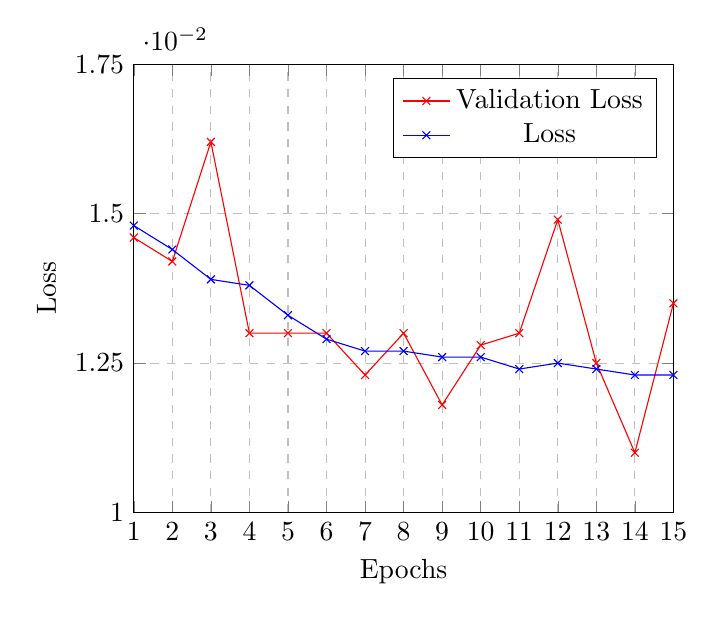
\begin{tikzpicture}
\begin{axis}[
    % title={Courbe de Loss en fonction des epochs},
    xlabel={Epochs},
    ylabel={Loss},
    xmin=1, xmax=15,
    ymin=0.01, ymax=0.0175,
    xtick={0,1,2,3,4,5,6,7,8,9,10,11,12,13,14,15},
    ytick={0.01,0.0125,0.015,0.0175,0.02},
    legend pos=north east,
    ymajorgrids=true,
    xmajorgrids=true,
    grid style=dashed
]

\addplot[
    color=red,
    mark=x,
    ]
    coordinates {
    (1,0.0146)(2,0.0142)(3,0.0162)(4,0.0130)(5,0.0130)(6,0.0130)(7,0.0123)(8,0.0130)(9,0.0118)(10,0.0128)(11,0.0130)(12,0.0149)(13,0.0125)(14,0.0110)(15,0.0135)
    };
    \addlegendentry{Validation Loss}
    
\addplot[
    color=blue,
    mark=x,
    ]
    coordinates {
    (1,0.0148)(2,0.0144)(3,0.0139)(4,0.0138)(5,0.0133)(6,0.0129)(7,0.0127)(8,0.0127)(9,0.0126)(10,0.0126)(11,0.0124)(12,0.0125)(13,0.0124)(14,0.0123)(15,0.0123)
    };
    \addlegendentry{Loss}    
\end{axis}
\end{tikzpicture}
\end{center}
\end{frame}

\begin{frame}
    \frametitle{Réseaux de neurones}
    \framesubtitle{Application au calcul du Flot Optique}
\begin{figure}[h]
        \centering
        \includegraphics[height=6cm]{Images/FlowNet/flownet_visualization_00001.png}
\end{figure}
Résultats obtenus pour un réseau simplifié.
\end{frame}

\begin{frame}
    \frametitle{Réseaux de neurones}
    \framesubtitle{Application au calcul du Flot Optique}
\begin{figure}[h]
        \centering
        \includegraphics[height=6cm]{Images/FlowNet/flownet_visualization_20000.png}
\end{figure}
Résultats obtenus pour un réseau simplifié.
\end{frame}

\section{Estimation de flot optique par apprentissage non-supervisé}
\begin{frame}
    \frametitle{Estimation de flot optique par apprentissage non-supervisé}
    Principe : on remplace la loss $AEE$, par une nouvelle loss : 
    \[\mathcal L(u,v,I(x,y,t),I(x,y,t+1))=\ell_{\text{photometric}}(u,v,I(x,y,t),I(x,y,t+1))\]
    \[+\lambda \ell_{\text{smoothness}}(u,v)\] 
    Où : \\
    \begin{itemize}
        \item $u,v\in\mathbb R^{H\times W}$  sont les composantes horizontales et verticales du flot prédit.
        \item $\ell_{\text{photometric}}(u,v,I(x,y,t),I(x,y,t+1))=\displaystyle\sum_{i,j}\rho_D(I(i,j,t)-I(i+u_{i,j},j+v_{i,j},t+1))$
        \item $\ell_{\text{smoothness}}(u,v)=\displaystyle\sum_{j}^{H}\sum_{i}^{W}(\rho_S(u_{i,j}-u_{i+1,j}) + \rho_S(u_{i,j}-u_{i,j+1})+\rho_S(v_{i,j}-v_{i+1,j}) + \rho_S(v_{i,j}-v_{i,j+1}))$
    \end{itemize}
    
\end{frame}

\begin{frame}
    \frametitle{Estimation de flot optique par apprentissage non-supervisé}
    Où : \\
    \begin{itemize}
        \item $\rho_{S,D}:x\mapsto(x^2+\varepsilon^2)^{\alpha_{S,D}}$ est la fonction de Charbonnier.
        \item $\lambda$ est un paramètre de régularisation qui décide de l'importance relative pour le flot prédit soit lisse ou non.
    \end{itemize}
    On garde ensuite l'architecture du modèle FlowNetSimple.
    
\end{frame}

\section{Conclusion et perspectives}
\begin{frame}
    \frametitle{Conclusion et perspectives}
    \begin{itemize}
        \item Résultats encourageants mais encore inutilisables car trop flous.
        \item On s'interesse à présent à l'apprentissage non-supervisé comme expliqué.
        \item Objectif : l'implémenter en Python
        \item L'appliquer aux matériaux
    \end{itemize}
\end{frame}

\end{document}
